\documentclass[]{article}
\usepackage{graphicx}
\usepackage{amsmath,amsfonts,amssymb}
\usepackage[many]{tcolorbox}
\usepackage[%
margin=2cm,
includefoot,
bottom=2.55cm,
top=2.025cm,
headsep=0.5cm,
footskip=0.65cm
]{geometry}

\definecolor{myblue}{RGB}{0,46,142}

\newtcolorbox[auto counter]{mytheorem}[1][]{%
	enhanced jigsaw,
	colback=white,
	colframe=myblue,
	coltitle=myblue,
	fonttitle=\bfseries,
	sharp corners,
	detach title,
	enlarge left by=18mm,
	width=\linewidth-18mm,
	underlay unbroken and first={%
		\node[above,text=myblue,font=\bfseries,align=center] at ([xshift=-.5\textwidth,yshift=-7mm]interior.north) {\thetcbcounter};
	},
	breakable,
	pad at break=1mm,
	#1,
	code={\ifdefempty{\tcbtitletext}{}{\tcbset{before upper={\tcbtitle\par\medskip}}}},
}
\graphicspath{ {./images/} }


%opening
\title{L-14: Orthogonal Vectors and Subspaces}
\author{Aahan Singh Charak\\Computer Science Grad}

\begin{document}

\maketitle

\section{Orthogonal Vectors}
\vspace{10pt}
\subsection{What are orthogonal vectors?}
Orthogonal vectors are vectors which lie at an angle of 90 degrees to each other. The dot product of such vectors is zero.\\

Consider two vectors at right angle to each other.
\vspace{12pt}
\begin{center}
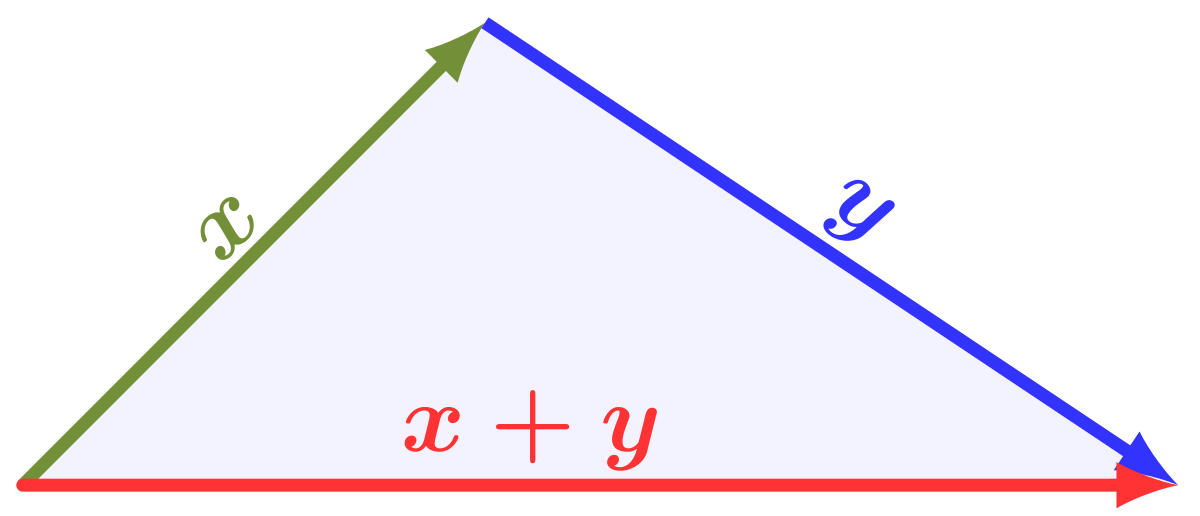
\includegraphics[scale=.25]{triangle}
\end{center}
\vspace{10pt}
Now, according to pythagoras:
\vspace{5pt}
$\|x\|^2 + \|y\|^2 = \|x+y\|^2$

This can be rewritten in vectoresque form as:\\

$x^Tx+y^Ty=(x+y)^T(x+y)$\\

$x^Tx+y^Ty=x^Tx+x^Ty+y^Ty+y^Tx$\\

$x^Ty+y^Tx=0$\\

$2x^Ty=0 \implies x^Ty=0$\\

This proves that dot product is zero for orthogonal vectors.

\subsection{Orthogonal Subspaces}

Two subspaces S and T are orthogonal, if and only if all vectors in S are orthogonal to all vectors in T.\\

\textbf{Note:} If two subspaces overlap (excluding zero vector), they are not considered as orthogonal subspaces; a vector cannot to orthogonal to itself.

\subsubsection{Row space is orthogonal to null space}
Why?\\

$x\in n(A)$\\

$Ax=0$\\

\[
\begin{bmatrix}
	a_{11} & a_{12} &...& a_{1n}\\
	a_{21}& a_{22} &...&a_{2n}\\
	...&...&...&...\\
	a_{m1}&a_{m2}&...&a_{mn}
	
\end{bmatrix}x=0
\]\\

Which means,\\
$row_1*x, row_2*x, row_3*x... row_m*x=0$\\

So, we get\\

$(\alpha_1*row_1+\alpha_2*row_2+...\alpha_m*row_m)x =0$\\

Therefore, \\

$Col-Space * x\in n(A) = 0$\\

Q.E.D

\subsubsection{Column space is orthogonal to null space of $A^T$}

Similar proof, do yourself.

\begin{mytheorem}[title=Important Note]
	Nullspace and rowspace are orthogonal complements in $R^n$.
\end{mytheorem}
\vspace{10pt}
\section{Solving Ax=b when there's no solution}
\vspace{10pt}
This problem might arise when there are more equations than the number of unknowns to be found. Bottom rows will be zero, as soon as we get n pivots. b might not have zeros in the last rows.

\subsection{Useful matrix for this}

Ax=b might not be solvable \\

$A^TA\hat{x}=A^Tb$ will have a solution\\

We get this using projections. Next lesson.\\


\begin{mytheorem}[title=Important Notes]
$N(A^TA)=N(A)$\\
$r(A^TA)=r(A)$\\
$A^TA$ is invertible only if A has independent columns.
\end{mytheorem}

\end{document}
